\section{State-of-the-Art}
	\tableofcontents[currentsection]
	
	\begin{frame}{High-Performance FPGA-Based CNN Accelerator With Block-Floating-Point Arithmetic}
		\centering
		\begin{figure}
			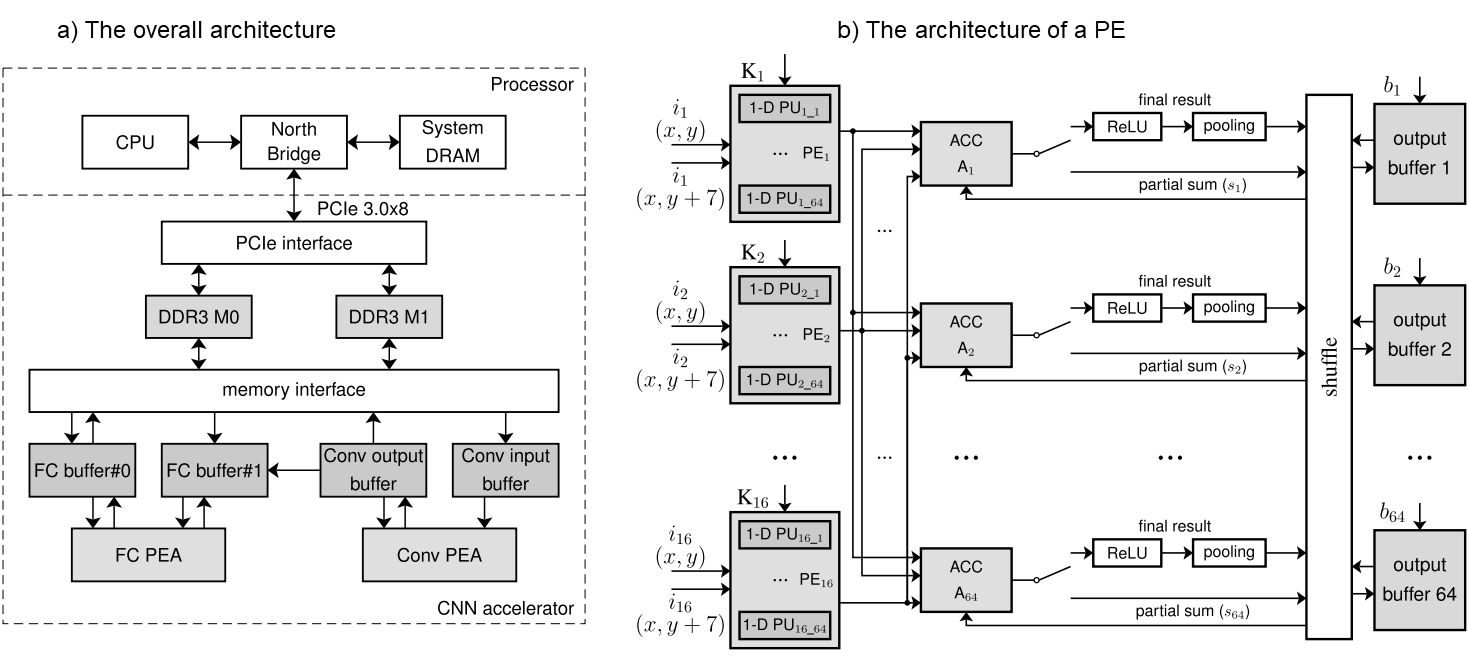
\includegraphics[width=\textwidth]{../figures/3_g.png}
			\caption{(a) System architecture. (b) Processing element array.}
		\end{figure}
	\end{frame}
	
	\begin{frame}{A 200MHZ 202.4GFLOPS@10.8W VGG16 Accelerator in Xilinx VX690T}
		\centering
		\begin{figure}
			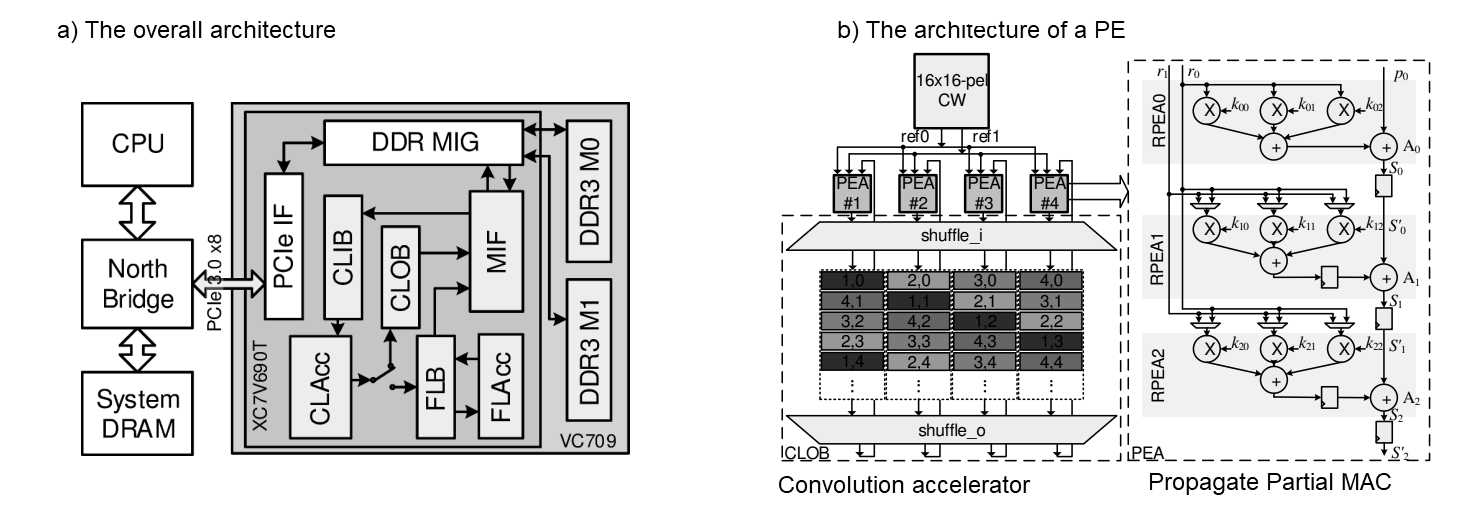
\includegraphics[width=\textwidth]{../figures/1_g.png}
			\caption{(a) System architecture. (b) Convolution accelerator.}
		\end{figure}
	\end{frame}
	
	\begin{frame}{Low-precision Floating-point Arithmetic for High-performance FPGA-based CNN Acceleration}
		\centering
		\begin{figure}
			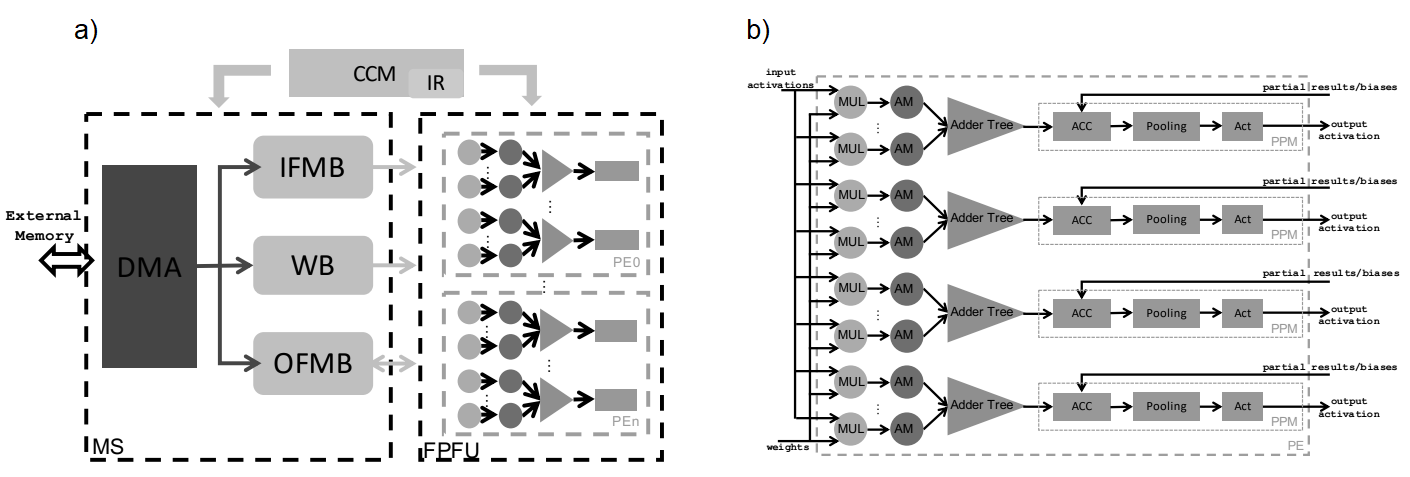
\includegraphics[width=\textwidth]{../figures/2_g.png}
			\caption{(a) System architecture. (b) Processing element.}
		\end{figure}
	\end{frame}

	\begin{frame}{CNN Hardware Acceleration on a Low-Power and Low-Cost APSoC}
	\centering
	\begin{figure}
		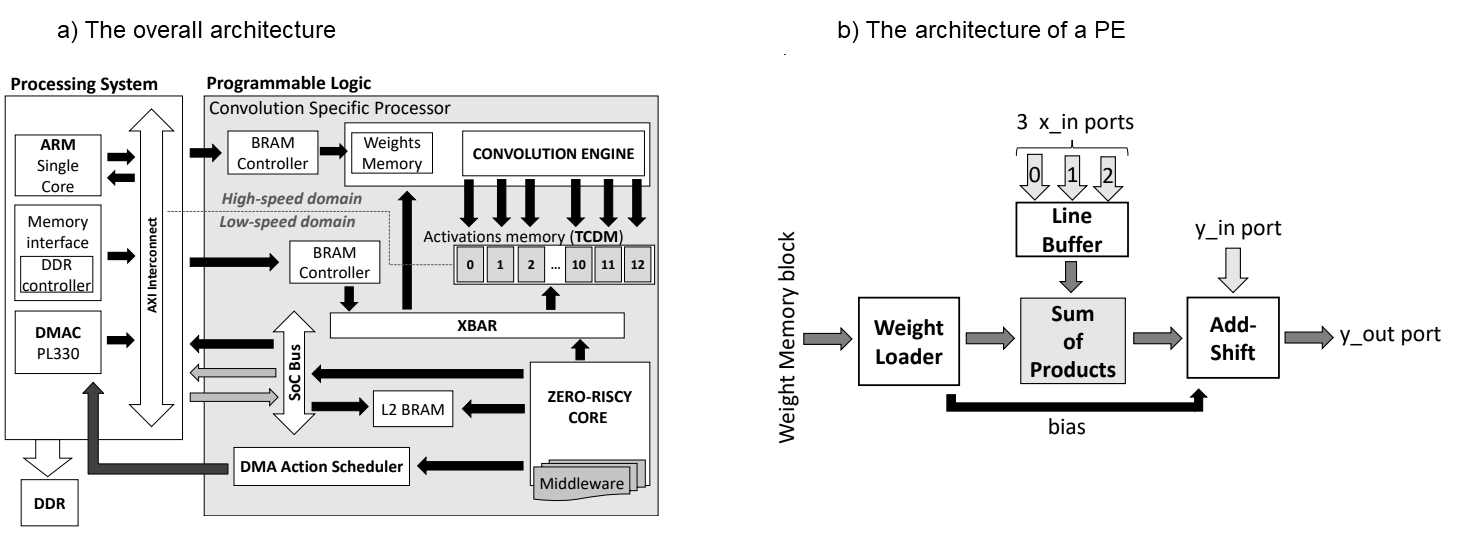
\includegraphics[width=\textwidth]{../figures/4_g.png}
		\caption{(a) System architecture. (b) Convolution engine.}
	\end{figure}
	\end{frame}